\documentclass{report}
\usepackage[utf8]{inputenc}
\usepackage[T1,T2A]{fontenc}
\usepackage[english,russian]{babel}
\usepackage{amsfonts}
\usepackage{amsmath}
\usepackage{upgreek}
\usepackage{amssymb}
\usepackage{wasysym}
\usepackage{graphicx}
\usepackage{amsthm}
\usepackage{hyperref}

\title{Проект по случайным графам}
\author{Чегодаева Таисия и Купряков Дмитрий, ПАДИИ, 2 курс}

\begin{document}
\maketitle

\part{Исследование свойств характеристики.}
\chapter{Исследовать, как ведет себя числовая характеристика $\tau$ в зависимости от параметров распределений $\theta$ и $\nu$, зафиксировав размер выборки и параметр процедуры построения графа.}
Замечание: ссылки на картинки пока что не кликабельные, но сами картинки лежат в той же папке, что и отчет.
\section{Характеристика $\tau^{KNN}$.}
\subsection{Распределение LogNormal с $\mu$ = 0 и параметром $\theta$.}
Зафиксируем размер выборки $n = 100$ и количество соседей $k = 5$. Число итераций для метода Монте-Карло равно 1000.
\newline
\newline
Будем перебирать $\theta \in (0, 1)$ и $\theta \in [1, 100]$.
\newline
\newline
\begin{figure}[h]
    \centering
    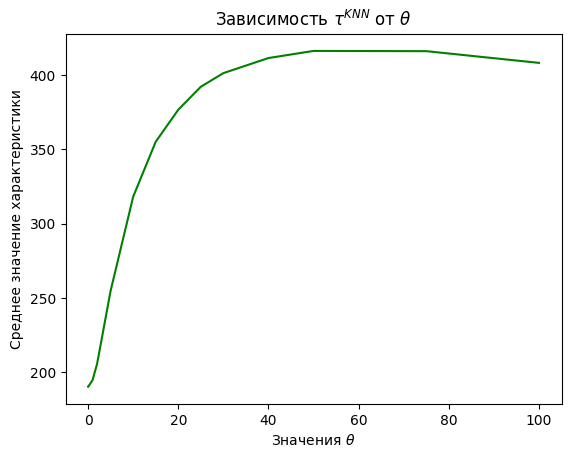
\includegraphics[width=0.5\linewidth]{2.png}
\end{figure}
\newline
\newline
Видно, что усредненная характеристика $\tau^{KNN}$ с увеличением $\theta$ растет. Возможно, график немного корявый и нужно посчитать характеристику при бОльших $\theta$, чтобы действительно был рост.
\newline
\newline
При этом на \texttt{1.png} видно, что при $\theta \in [0, 1]$ значение характеристики колеблется около 189-190.

\subsection{Распределение Exp с параметром $\lambda$.}
Зафиксируем размер выборки $n = 100$ и количество соседей $k = 5$. Число итераций для метода Монте-Карло равно 1000.
\newline
\newline
Точно также будем перебирать $\nu \in (0, 1)$ и $\nu \in [1, 100]$.
\newline
\newline
\begin{figure}[h]
    \centering
    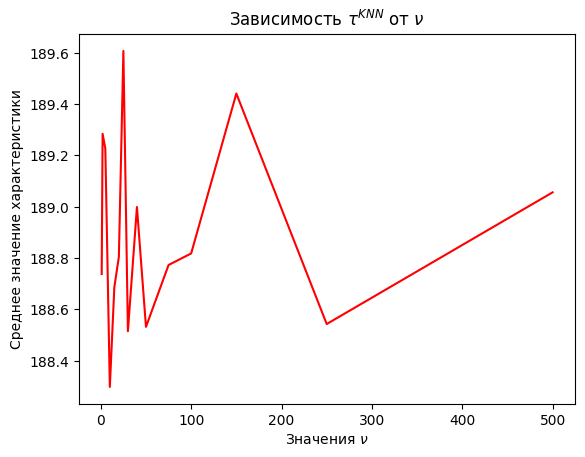
\includegraphics[width=0.5\linewidth]{4.png}
\end{figure}
\newline
\newline
Усредненная характеристика $\tau^{KNN}$ принимает значения в окрестности числа 189 независимо от параметра $\nu$.

\section{Характеристика $\tau^{dist}$.}
\subsection{Распределение LogNormal с $\mu$ = 0 и параметром $\theta$.}
Зафиксируем размер выборки $n = 100$ и расстояние $dist = 5$. Число итераций для метода Монте-Карло равно 1000.
\newline
\newline
Будем перебирать $\theta \in (0, 1)$ и $\theta \in [1, 1000]$.
\newline
\newline
\begin{figure}[h]
    \centering
    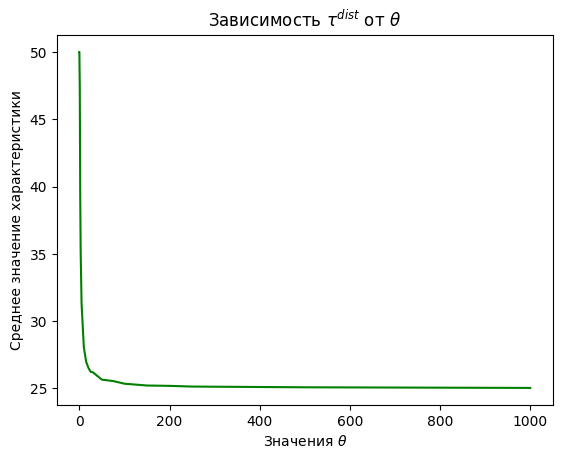
\includegraphics[width=0.5\linewidth]{6.png}
\end{figure}
\newline
\newline
Характеристика $\tau^{dist}$ при $\theta \in (0, 1)$ принимает значение 50 (т.е. при таких $\theta$ граф -- полный). 
\newline
\newline
При $\theta \in [1, +\infty)$ с увеличением $\theta$ среднее значение характеристики $\tau^{dist}$ колеблется в окрестности числа 25.
\newline
\newline
Дополнительно смотрела на большие $\theta \in [15, 500000]$, начиная с некоторого момента нижняя граница колебаний $\tau^{dist}$ выравнивается (как раз где-то до $\tau^{dist} = 25$), соотвественно, среднее значение немного увеличивается и колеблется около 27.

\subsection{Распределение Exp с параметром $\lambda$.}
Зафиксируем размер выборки $n = 100$ и расстояние $dist = 5$. Число итераций для метода Монте-Карло равно 1000.
\newline
\newline
Будем перебирать $\nu \in (0, 1)$ и $\theta \in [1, 1000]$.
\newline
\newline
\begin{figure}[h]
    \centering
    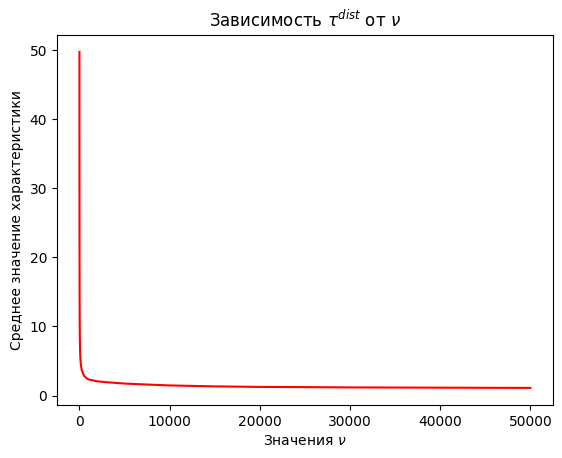
\includegraphics[width=0.5\linewidth]{8.png}
\end{figure}
\newline
\newline
Характеристика $\tau^{dist}$ при $\nu \in (0, 1)$ принимает значение 50 (т.е. при таких $\nu$ граф -- полный). 
\newline
\newline
При больших $\nu$ среднее значение $\tau^{dist}$ стремится к 1.
\newline
\newline
Замечание: для экспоненциального распределения видно более резкое уменьшение значения характеристики по сравнению с lognormal распределением.

\chapter{Исследовать, как ведет себя числовая характеристика $\tau$ в зависимости от параметров процедуры построения графа и размера выборки при фиксированных значениях $\theta = \theta_0$ и $\nu = \nu_0$.}
\section{Характеристика $\tau^{KNN}$.}
\subsection{Распределение LogNormal с $\mu$ = 0 и $\theta = \theta_0 = 1$ + распределение Exp с параметром $\nu = \nu_0 = \frac{1}{\sqrt{e^2 - e}}$.}
Картинку смотрите тут: \texttt{11.png}.
\newline
\newline
Замечания:
\newline
\newline
- $\tau^{KNN}$ для Exp распределения растет медленнее, чем для LogNormal распределения.
\newline
\newline
- Стоит посмотреть на значения характеристики при бОльших размерах выборки (еще не смотрела), т.к. кажется, что при увеличении выборки найти границу, может быть, получится.
\newline
\newline
Возможно, еще добавлю что-то сюда.

\section{Характеристика $\tau^{dist}$.}
\subsection{Распределение LogNormal с $\mu$ = 0 и $\theta = \theta_0 = 1$ + распределение Exp с параметром $\nu = \nu_0 = \frac{1}{\sqrt{e^2 - e}}$.}
Картинку смотрите тут: \texttt{14.png}.
\newline
\newline
Пара замечаний:
\newline
\newline
- $\tau^{dist}$ для Exp распределения растет быстрее, чем для LogNormal распределения.
\newline
\newline
- $dist \ge 50$ можно не рассматривать, т.к. для обоих распределений характеристика показывает одинаковое значение (хроматическое число равно числу вершин).
\newline
\newline
- есть подозрение, что если $\tau^{dist} \ne n$, где $n$ -- число вершин в графе при $dist \in [5, 50]$, то очень вероятно, что этот граф был построен на реализациях случайной величины lognormal распределения.
\newline
\newline
- пока что $\tau^{dist}$ рассматривать и изучать приятнее/проще, чем $\tau^{KNN}$.

\chapter{Построить множество A в предположении $\theta = \theta_0$ и $\nu = \nu_0$ при максимальной допустимой вероятности ошибки первого рода $\alpha = 0.05$. Оценить мощность полученного критерия.}
\section{Характеристика $\tau^{KNN}$.}
Для визуализаций смотрите картинку \texttt{15.png}.
\newline
\newline
Распределения смешаны между собой, и невозможно определить какую-либо границу между ними. Выходит, что работать с KNN-графом довольно трудно. Посмотрим на дистанционный граф. 
\newline
\newline
Но я все-таки хотела бы посмотреть на KNN-граф на большом числе вершин и уже после этого определиться с ответом.

\section{Характеристика $\tau^{dist}$.}
Для визуализаций смотрите картинку \texttt{16.png}.
\newline
\newline
А вот тут четко просматривается граница между двумя распределениями, особенно при бОльших размерах выборки. Построим множество $A$ (синие пунктирные линии на графике).
\newline
\newline
Для визуализаций смотрите картинку \texttt{17.png}.
\newline
\newline
При увеличении $dist$ и размера выборки граница между двумя распределениями становится более явной. И даже есть примеры, когда мощность максимальна и равна 1.
Однако при небольших размерах выборки и маленьких $dist$ распределения довольно трудно различимы.
\newline
\newline
\emph{Вывод:} если дана выборка достаточного размера, то при выборе правильного $dist$ ($\approx 5$) можно построить дистанционный граф так, что по хроматическому числу этого графа будет возможно определить исходное распределение.

\end{document}
